\documentclass[tikz, border=2pt]{standalone}

\usepackage{helvet}
\renewcommand{\familydefault}{\sfdefault}

\usepackage[EULERGREEK]{sansmath}
\sansmath
\usetikzlibrary{arrows.meta}

\begin{document}%

\begin{tikzpicture}[line width=2pt]
\tikzset{>={Latex[width=3mm,length=4mm]}}

% % grid
% \draw[help lines] (-0.5, -5) grid (13, 18);


\node[inner sep=0pt] (figa) at (10.5,12)
{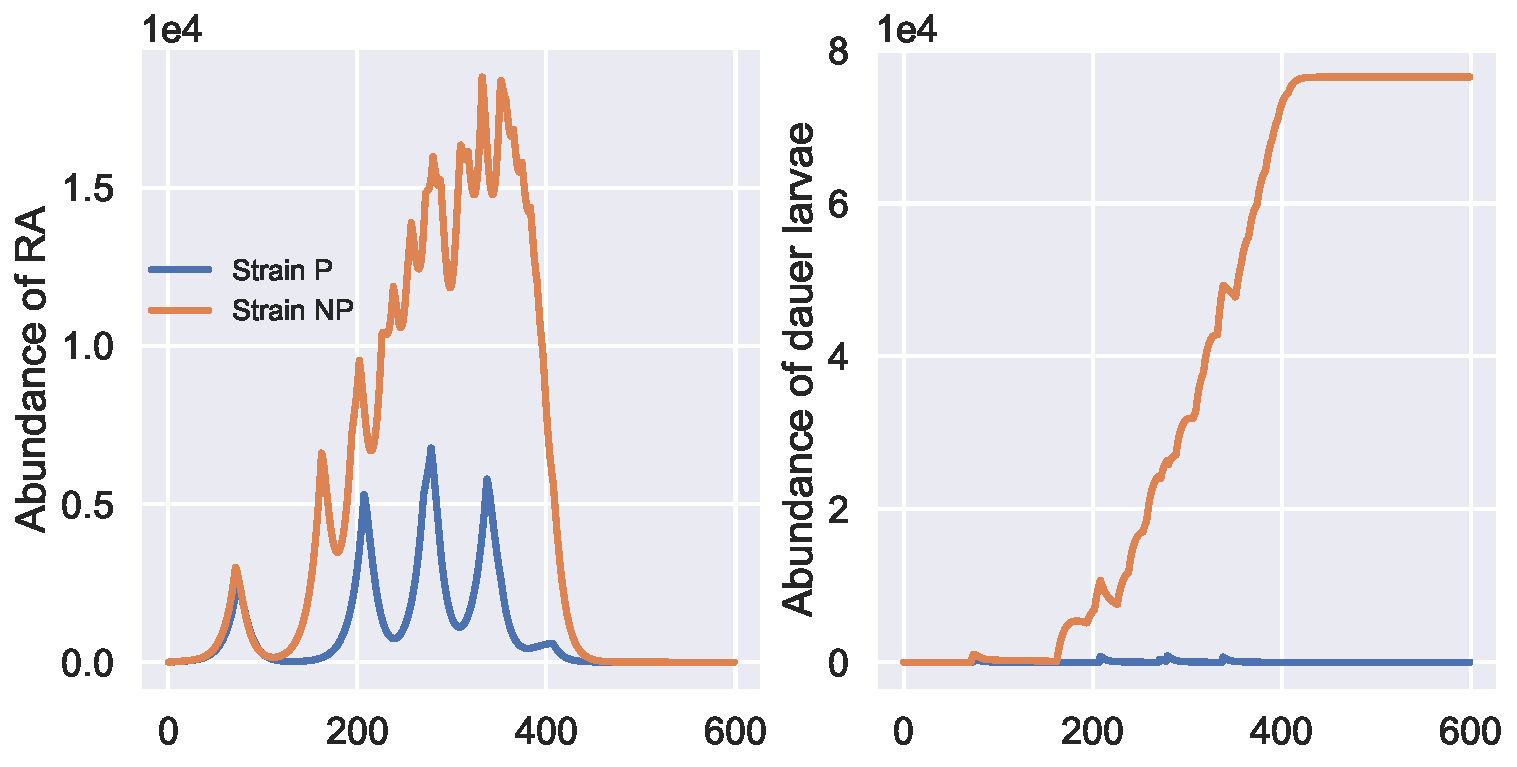
\includegraphics[width=1.\textwidth]{../meta_quad_1.pdf}};

\node[inner sep=0pt] (figa) at (2.5,12)
{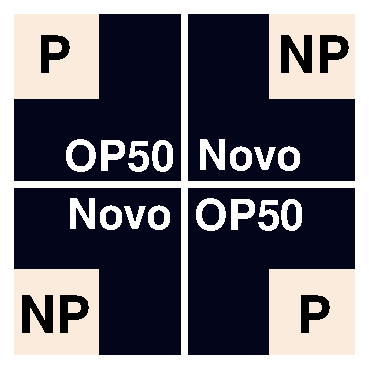
\includegraphics[width=0.3\textwidth]{./tikz_figs/pop_icon_quad_1.pdf}};

\node[inner sep=0pt] (figa) at (10.5,5)
{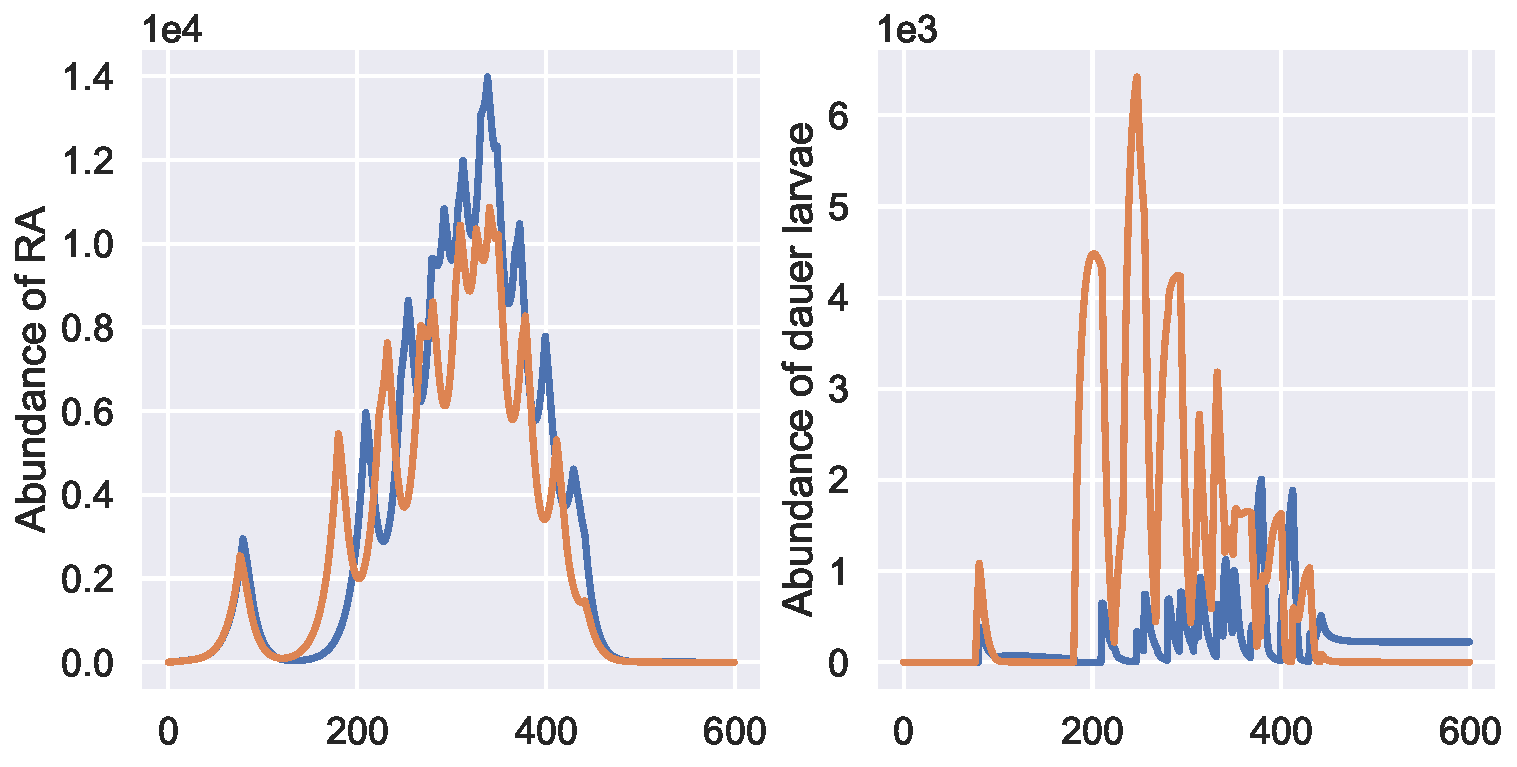
\includegraphics[width=1.\textwidth]{../meta_quad_2.pdf}};

\node[inner sep=0pt] (figa) at (2.5,5)
{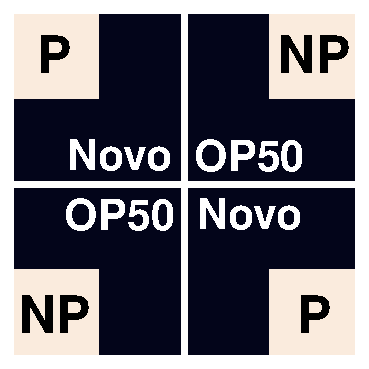
\includegraphics[width=0.3\textwidth]{./tikz_figs/pop_icon_quad_2.pdf}};


% %labels
\draw (0., 14.8) node{{\Huge\sf\textbf{a}}};

\draw (0., 8) node{{\Huge\sf\textbf{b}}};

% \draw (10.3, 14.8) node{{\Huge\sf\textbf{b}}};

% \draw (10.3, 10.3) node{{\Huge\sf\textbf{c}}};

% \draw (0., 6.3) node{{\Huge\sf\textbf{d}}};

% \draw (0., 11.5) node{{\Huge\sf\textbf{c}}};

% \draw (0., 6.3) node{{\Huge\sf\textbf{d}}};


\end{tikzpicture}


\end{document}